% !TEX encoding = UTF-8
% !TEX TS-program = pdflatex
% !TEX root = ../tesi.tex

%**************************************************************
\chapter{Contesto aziendale}
\label{cap:introduzione}
%**************************************************************

%**************************************************************
\section{Lab Network}
\lab{} nasce nel 2016 con lo scopo di aiutare le imprese a creare e ad innovare prodotti e processi attraverso la competenza concreta dei laboratori, sfruttando le potenzialità dei moderni strumenti digitali.\\
Nel dettaglio \lab{} offre la possibilità di importanti avanzamenti tecnologici a PMI offrendo servizi di consulenza oltre che ricerca e sviluppo di progetti sperimentali.\\
L'azienda cerca di collaborare con più partner per poter ottenere una visione maggiore di prodotti e di conseguenza soddisfare i clienti.\\
L'ambiente lavorativo è condiviso con un'altra azienda: \textit{Business Research Srl}, la quale si occupa di soluzioni software su misura, applicazioni per aziende, e-commerce, cloud e hosting.\\
Tra le due aziende è in vigore un accordo che le lega in una stretta collaborazione: infatti, nel periodo di sviluppo di un nuovo progetto, Business Research si occupa della parte software.\\
Durante lo stage ho di fatto interagito con il personale di quest'ultima azienda per la realizzazione del progetto.

\section{Organizzazione aziendale}
\subsection{Contesto lavorativo}
\lab{} è un'azienda giovane ma intraprendente e farne parte significa entrare in un gruppo eterogeneo di aziende che collaborano per un fine comune.\\
L'azienda opera principalmente nel territorio Veneto, cercando di coinvolgere le PMI del territorio in un processo di aggiornamento tecnologico seguendo tre fasi:
\begin{itemize}
\item Creare l'interesse attraverso politiche di marketing discutendo di temi specifici ad alto impatto mediatico;
\item Raccogliere gruppi omogenei che condividono l'interesse ad una specifica tecnologia;
\item Capire le esigenze produttive e le potenzialità che una digitalizzazione (hardware o software) può contribuire alla crescita di una PMI, attraverso attività di consulenza e formazione.
\end{itemize}
Il ruolo più importante di \textit{business scouting} è affidato al \textbf{dirigente aziendale}, che si occupa quindi della valutazione di idee imprenditoriali, valutandone la fattibilità.\\
La \textbf{segreteria} ha il compito organizzativo per quanto riguarda appuntamenti e gestione di eventi (fiere, presentazioni, convegni, ecc.) oltre che quello di relazione con i clienti.\\
L'\textbf{amministrazione} si occupa della gestione dell'aspetto finanziario dell'azienda: fatturazione, pagamenti e rapporti con le banche.\\
Il \textbf{team di sviluppo} viene creato di volta in volta in collaborazione con Business Research Srl, che fornisce le risorse umane.\\
\\
Dal momento in cui una PMI decide di investire in un aggiornamento tecnologico attraverso l'introduzione di un nuovo prodotto o servizio, \lab{} per prima cosa sviluppa un piano di lavoro che prevede una prima fase di ricerca, seguita poi dalla realizzazione vera e propria.\\
Nella fase di ricerca \lab{} coinvolge varie aziende specializzate creando così una rete di imprese che collaborano per portare a termine il progetto innovativo, oggetto della ricerca.\\
\\
Durante il periodo di stage ho potuto conoscere come lavora il team di sviluppo: viene adottata una metodologia di tipo agile, ciò consente di avere un dialogo continuo con il cliente che può decidere di modificare il progetto in corso d'opera.\\
Ho appreso inoltre che il team fa riferimento al framework scrum per la gestione dei processi e dei ruoli.

\section{Prodotti e servizi}
\subsection{Prodotti}
\textbf{VITRUVIAN GAME – Wingsuit VR}
\\
Si tratta di un progetto nato dalla collaborazione con Intel\textsuperscript{\textregistered} e rappresenta un simulatore di volo con tuta alare.\\
La sua forma è ispirata all'\textit{Uomo Vitruviano} di Leonardo da Vinci.\\
Il progetto prevede l'utilizzo del visore HTC Vive affiancato ad uno scenario virtuale sviluppato con motore grafico \textit{Unreal Engine}. Per i movimenti sugli assi sono stati impiegati dei motori per automazione industriale.\\
L'utente può controllare i movimenti tramite dei controller posti su entrambe le mani.
\\
\begin{figure}[H]
	\begin{center}
	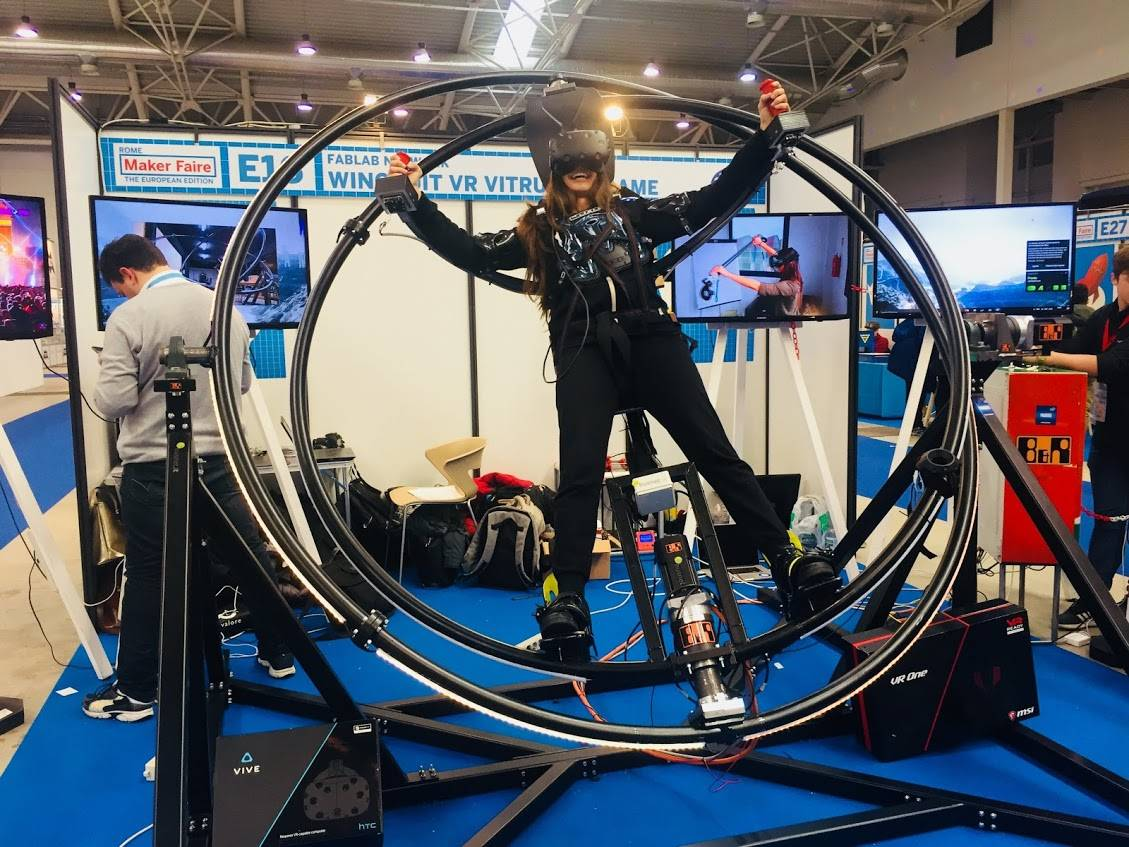
\includegraphics[scale=0.15]{immagini/vitruvian.jpg}
	\caption{Vitruvian Game - Il simulatore di volo con tuta alare}
	\end{center}
\end{figure}

\noindent \textbf{FabKey}
\\
FabKey è una serratura smart composta da un sistema di controllo connesso ad internet che permette l'apertura di una porta, andando a verificare una lista di accessi presente in cloud. Funziona tramite lettura di tag \gls{NFC} o barcode. Il prodotto è rivolto principalmente ai \gls{FabLab}, ma si adatta facilmente a qualsiasi contesto in cui sia richiesto il controllo degli accessi.\\
Le principali tecnologie utilizzate in questo prodotto sono Arduino e relativa programmazione in C/C++ per la parte hardware, mentre per il software crm sono stati utilizzati linguaggi come Html, Javascript, NodeJS, CSS ecc.
\\
\begin{figure}[H]
	\begin{center}
	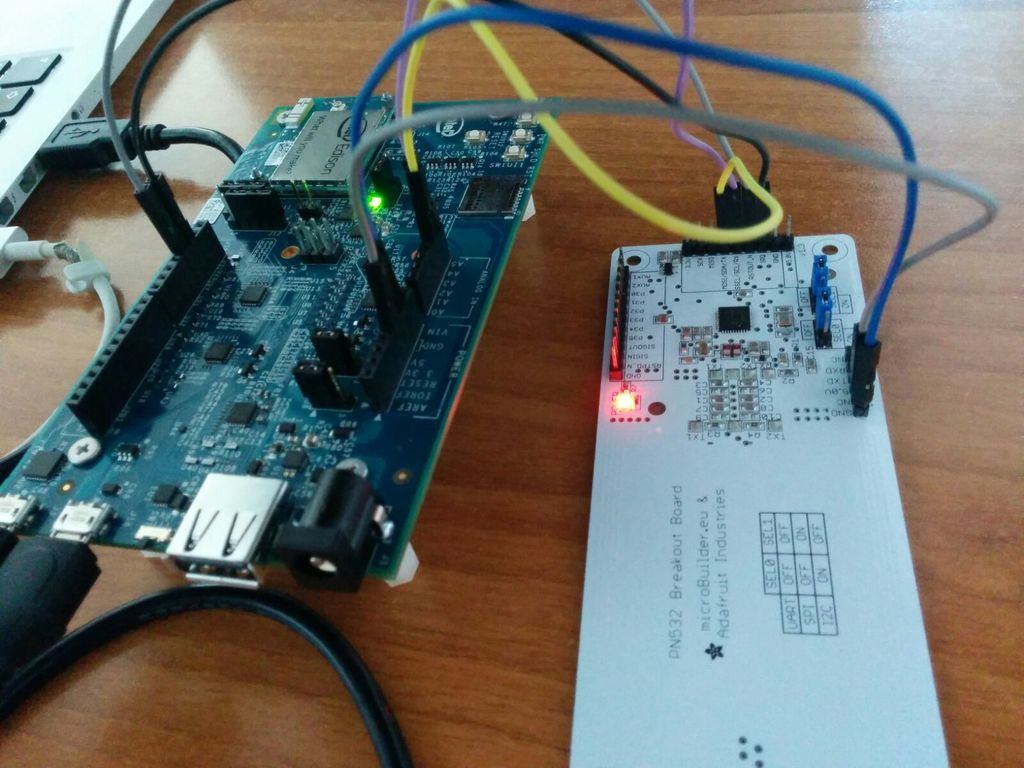
\includegraphics[scale=0.2]{immagini/fabkey.jpg}
	\caption{Prototipo di FabKey durante la fase di programmazione}
	\end{center}
\end{figure}

\noindent \textbf{Smart Meter}
\\
Un metro intelligente dotato di rotella metrica ed encoder ottico, capace di misurare superfici complesse e inviare direttamente i dati al software gestionale, in aggiunta anche il monitoraggio in tempo reale di quando, dove e per quanto tempo è stato utilizzato dal singolo addetto.\\
Il dispositivo è stato sviluppato sulla base di schede elettroniche programmabili open source.
\\
\begin{figure}[H]
	\begin{center}
	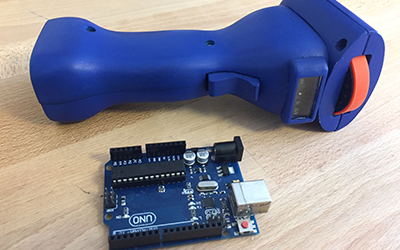
\includegraphics[scale=0.6]{immagini/smartmeter.png}
	\caption{Smart Meter: il metro intelligente}
	\end{center}
\end{figure}

\subsection{Servizi}
Il servizio principale che \lab{} offre ai propri clienti è quello di accompagnare le aziende in un percorso di aggiornamento tecnologico, fornendo supporto in termini di tecnologie e conoscenze.
Durante l'esperienza di stage ho potuto verificare i passaggi che caratterizzano questo servizio:
\begin{itemize}
\item Analisi dettagliata delle esigenze del cliente, tramite diversi incontri con gli stakeholders;
\item Studio di fattibilità grazie ad un'attenta analisi di mercato;
\item Progettazione e/o implementazione dell'innovazione di processo o prodotto lavorando in sinergia con le aziende partner che più si avvicinano alle materie trattate.
\end{itemize}
Altri servizi che \lab{} offre ai propri clienti sono:
\begin{itemize}
\item \textbf{Didattica:} corsi di formazione su misura, \gls{counseling} e \gls{workshop} per imparare a sfruttare in modo professionale: stampa 3D, schede elettroniche, realtà virtuale e aumentata, sviluppo applicazioni, prototipazione, \gls{bigd}, \gls{iot} ecc.
\item \textbf{Noleggio:} kit e attrezzature come stampanti 3D, schede elettroniche (\gls{arduino}, \gls{rpi}, Intel) visori VR, pc e notebook, videoproiettori; affitto di aule didattiche;
\item \textbf{Personale qualificato:} per i clienti sono a disposizione docenti, tecnici di laboratorio e consulenti specializzati nei principali ambiti di innovazione digitale.
\end{itemize}

\subsection{Tecnologie}
L'intero team utilizza ambienti con sistema operativo \textit{macOS} per le attività di sviluppo. 
\subsubsection{Elettronica e Hardware}
A supporto dei processi di prototipazione, \lab{} utilizza diverse piattaforme hardware come ad esempio \textit{Arduino}, \textit{Raspberry Pi}, \textit{Intel UP Square}, \textit{Asus TinkerBoard}.\\
La programmazione delle schede Arduino avviene tramite l'omonimo ambiente di sviluppo integrato, con linguaggi C/C++.\\
\lab{}, inoltre, sfrutta le potenzialità della stampa 3D e del disegno CAD per creare modelli prototipali in modo rapido. La disponibilità in azienda di 3 stampanti 3D permette di ridurre il tempo per la realizzazione dei prototipi da proporre al cliente.\\
Tali tecnologie sono state ampiamente utilizzate per lo sviluppo di progetti come FabKey e SmartMeter, soprattutto in fase di sperimentazione e prototipazione.

\begin{figure}[H]
	\begin{center}
	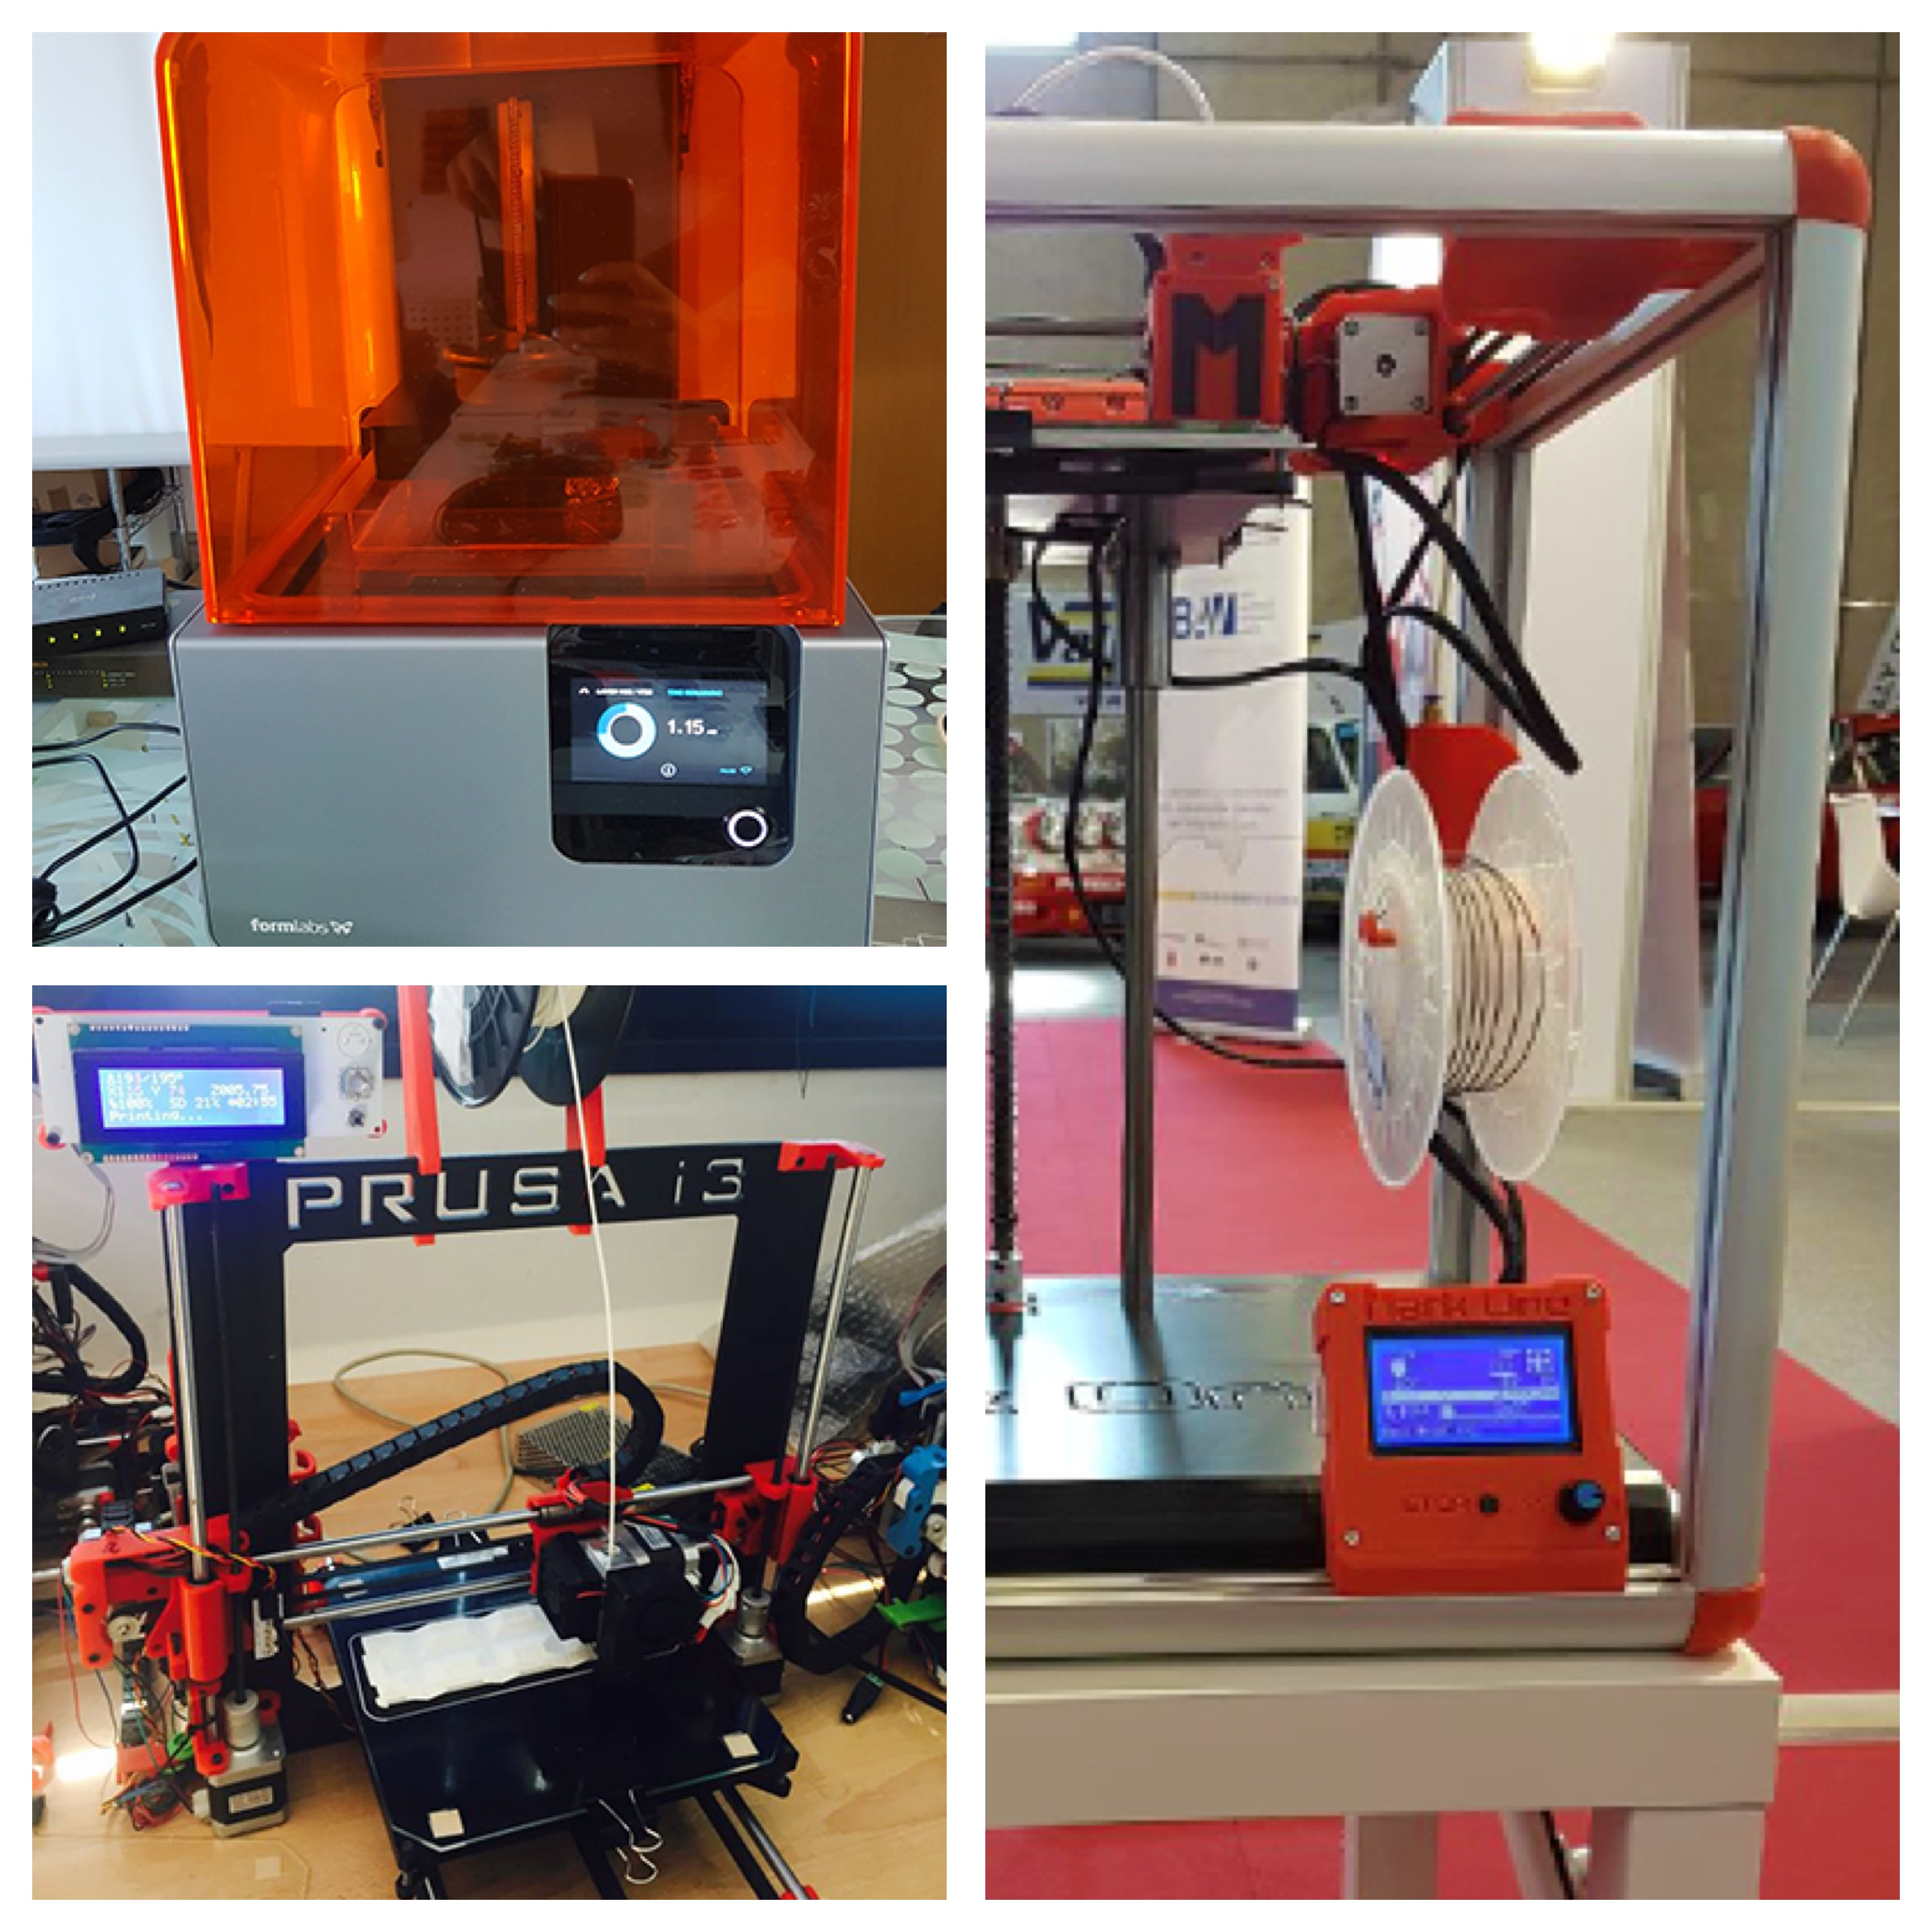
\includegraphics[scale=0.08]{immagini/stampanti.jpg}
	\caption{Le stampanti 3D in dotazione a \lab{}}
	\end{center}
\end{figure}

\subsubsection{Realtà virtuale e aumentata}
L'azienda utilizza software e strumenti per lo studio e lo sviluppo in ambito della realtà virtuale ed aumentata.
Nel dettaglio, è stato utilizzato il motore grafico \textit{Unreal Engine} per lo sviluppo dell'ambiente virtuale relativo al Vitruvian Game: per utilizzare e testare tale ambiente, \lab{} utilizza il visore \textit{Vive} prodotto da \textit{HTC}.\\
L'azienda, in ambito di realtà aumentata, utilizza la piattaforma \textit{Unity} per lo sviluppo di nuove applicazioni.\\

\begin{figure}[H]
	\begin{center}
	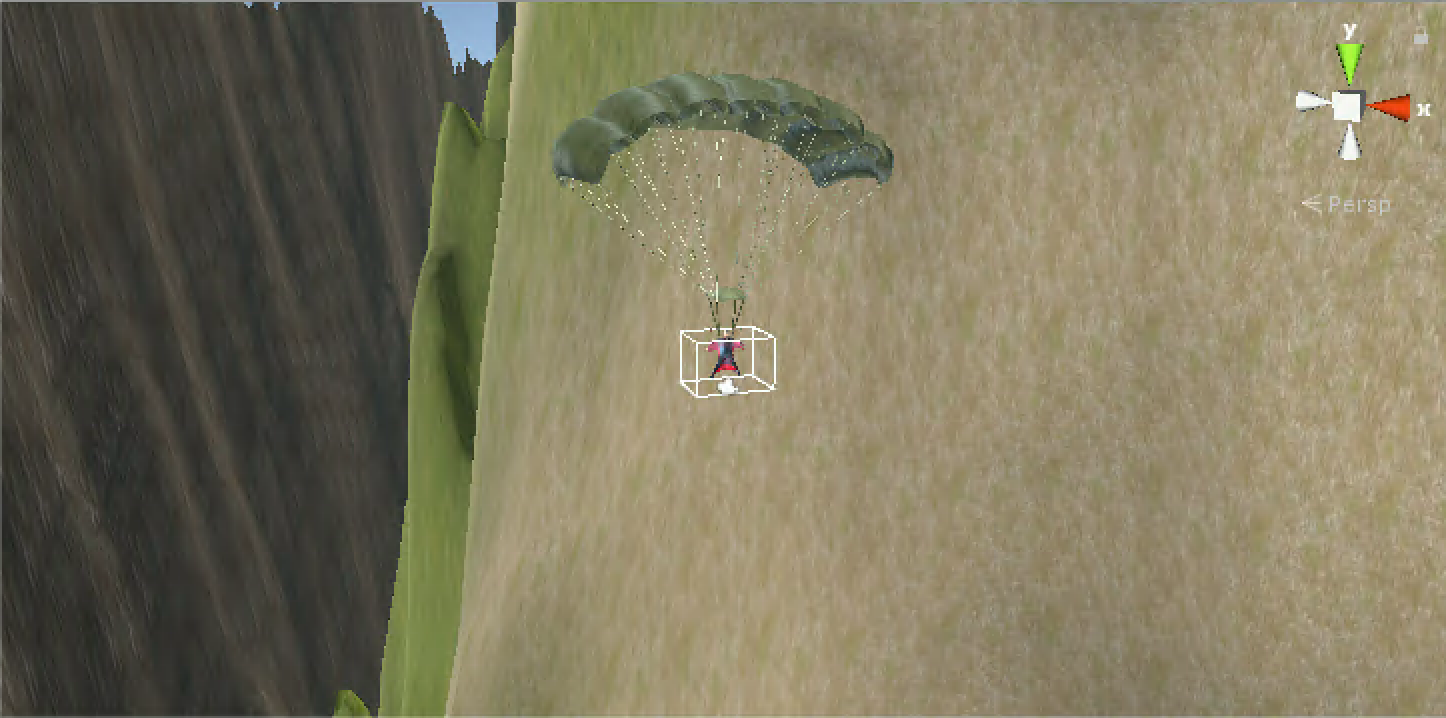
\includegraphics[scale=0.22]{immagini/unity.png}
	\caption{L'ambiente virtuale realizzato con Unreal Engine durante la fase di sviluppo}
	\end{center}
\end{figure}

\subsubsection{Tecnologie di supporto}
A supporto dei processi di sviluppo, l'azienda utilizza la piattaforma web di \textit{GitLab}, che consente la gestione di repository Git e di funzioni trouble ticket.\\
L'utilizzo di questa piattaforma permette il controllo della configurazione e del versionamento di un software, oltre che la gestione di ticket.\\
Come detto in precedenza, la piattaforma viene utilizzata anche per la gestione del Product Backlog.

\subsubsection{Sviluppo web}
Alcuni progetti richiedono lo sviluppo di applicazioni web: nel caso di FabKey è stato realizzato un software per la gestione delle autorizzazioni e il controllo degli accessi nei determinati varchi.\\
Tale applicazione web è stata sviluppata utilizzando PHP e MySQL per la parte backend, mentre HTML, CSS e JavaScript per la parte frontend.

\subsubsection{Deep Learning e intelligenza artificiale}
Intel Movidius è un prodotto di apprendimento profondo che permette di far girare reti neurali profonde in tempo reale direttamente dal dispositivo, consentendo di svolgere un'ampia gamma di applicazioni IA offline.\\
Utilizzando questa tecnologia, \lab{} sta attualmente sviluppando un progetto che consiste nella previsione di futuri incidenti e infortuni sul lavoro.\\
Sfruttando le tecniche di \textit{deep learning} messe a disposizione dall'hardware e analizzando grandi dati riguardanti incidenti passati, si è in grado di effettuare una stima sui possibili incidenti futuri.
\begin{figure}[H]
	\begin{center}
	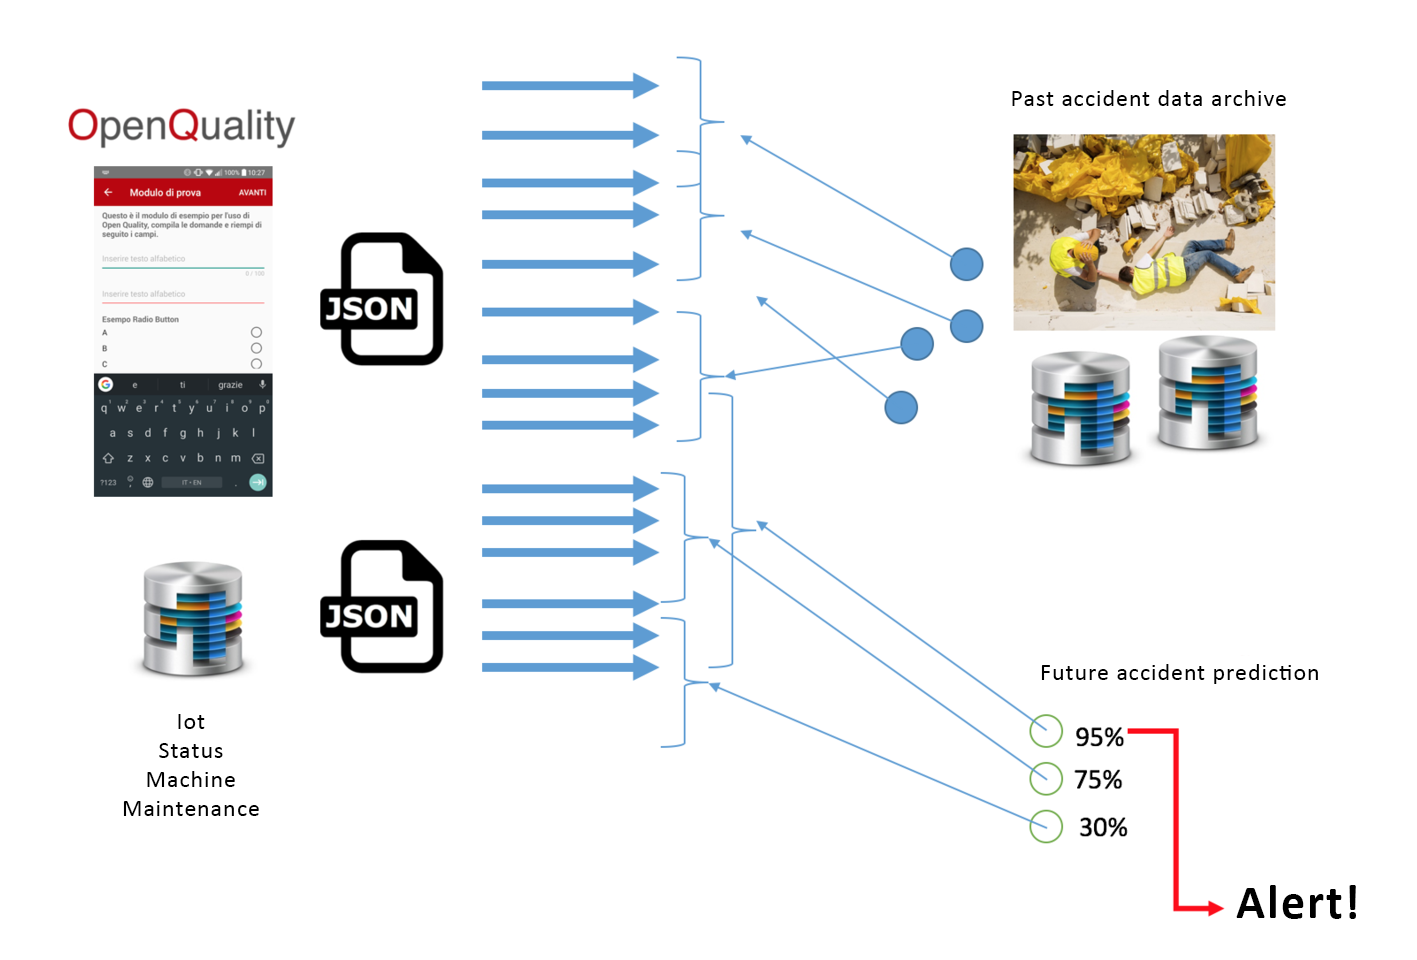
\includegraphics[scale=0.25]{immagini/accident_prediction.png}
	\caption{Previsione degli infortuni sul lavoro: schema di funzionamento}
	\end{center}
\end{figure}

\section{Lab Network e innovazione}
\subsection{Pensiero aziendale}
\lab{} si è sviluppata nell'ambito della \textit{smart specialisation} attraverso logiche di coinvolgimento di una comunità di utenti misti che provengono prevalentemente dal mondo aziendale e accademico. 
L'azienda si propone come punto di riferimento per l'innovazione \textit{Open Source} del Veneto, promuovendosi come centro privilegiato di interscambio di conoscenza.\\
Come previsto dalla Smart Specialisation Strategy, è stata condotta una prima fase di analisi dall'azienda ed è emerso che il territorio regionale è composto principalmente da piccole e medie imprese di tipo manifatturiero. Sulla base di ciò, \lab{} si è posta l'obiettivo di contribuire, attraverso strumenti e modalità di funzionamento specifici, a sviluppare ed attuare la strategia regionale della ``Fabbrica Intelligente Del Futuro''.\\
Questa mira ad indirizzare la trasformazione del settore manifatturiero verso nuovi prodotti, processi e tecnologie, attraverso lo sviluppo di attività di ricerca di alto livello.\\
Per questo \lab{} è sempre alla ricerca di nuove tecnologie, in modo da essere sempre aggiornata 

\subsection{Smart Specialisation Strategy}
\begin{figure}[H]
	\begin{center}
	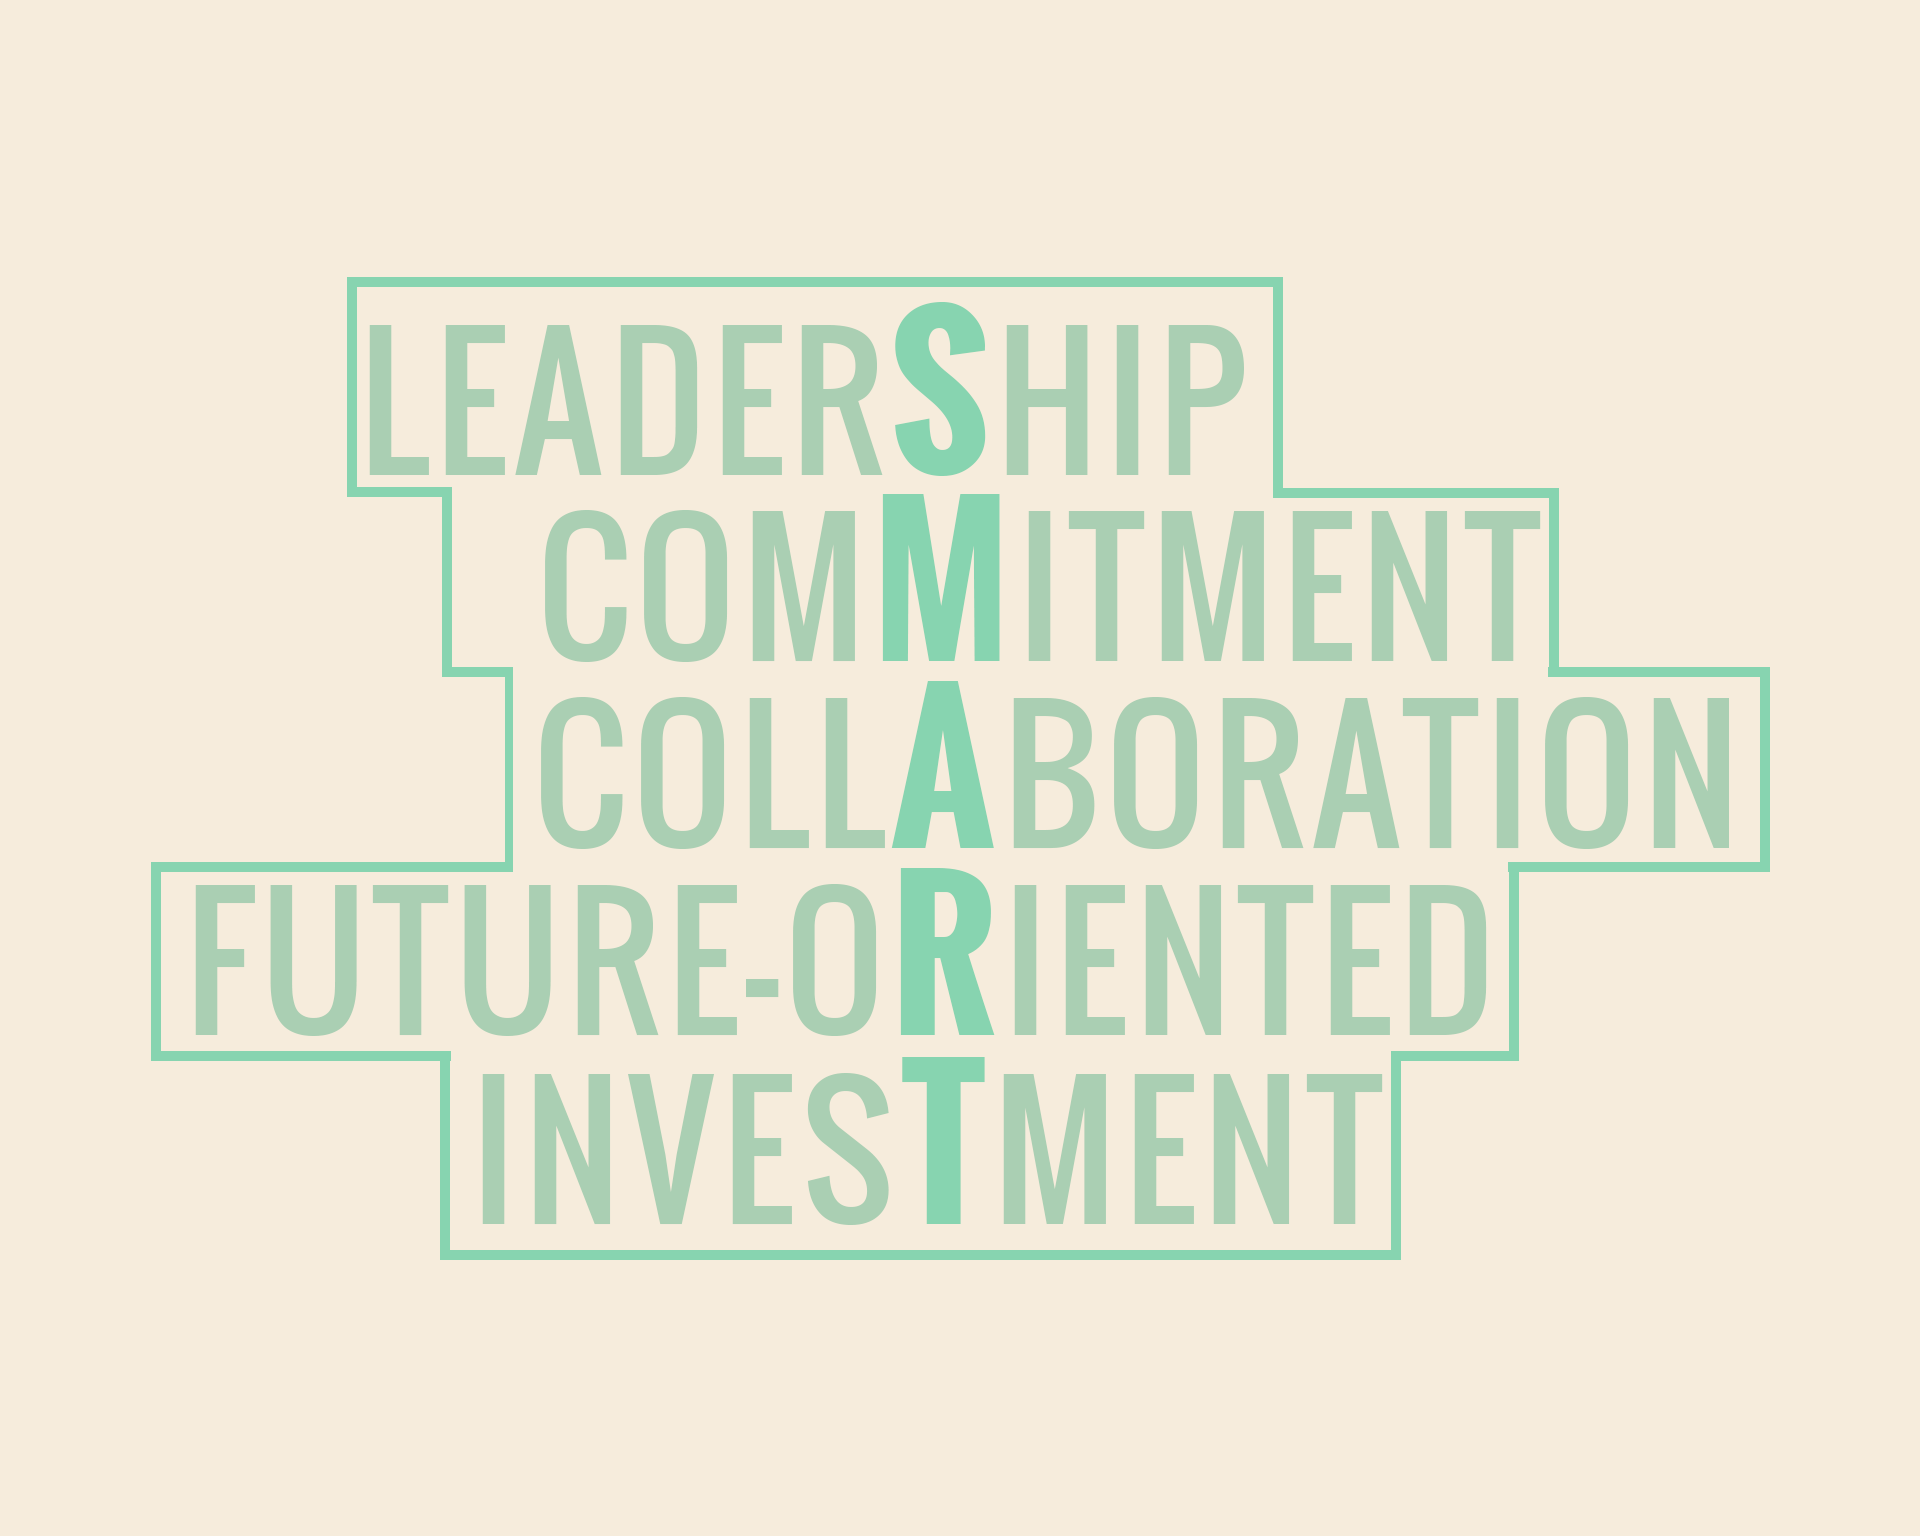
\includegraphics[scale=0.15]{immagini/SMART.png}
	\caption{Punti chiave della Smart Specialisation Strategy. Video \textit{"The Kingdom of Smart"}.
	\small{\textbf{Fonte:} \url{http://s3platform.jrc.ec.europa.eu/home}}		
				}
	\end{center}
\end{figure}

\begin{flushright}{
	\slshape    
	``L'innovazione non può essere dettata, ma può essere coltivata attraverso scoperte imprenditoriali; ciò richiede una leadership, un impegno comune sostenuto tramite collaborazione e investimenti orientati al futuro.''} 
	
	\medskip
    --- \textit{Pubblicità progresso, Commissione Europea - 2013}
\end{flushright}

% Vedi link: https://www.researchitaly.it/smart-specialisation-strategy/
% Utile: https://www.slideshare.net/TCINetwork/8-clac-18-junefrederic-miribel

\noindent La \textit{Smart Specialisation Strategy} (S.S.S.) è una strategia concepita nell'ambito della politica di coesione riformata dalla Commissione Europea per incentivare l'innovazione regionale al fine di ottenere una crescita economica, permettendo alle regioni di focalizzare i loro punti di forza..\\
Delinea delle strategie di innovazione concepite a livello regionale ma messe a sistema a livello nazionale con l'obiettivo di:
\begin{itemize}
\item sviluppare strategie di innovazione a livello regionale, mirate a valorizzare ambiti produttivi di eccellenza, considerando il posizionamento strategico all'interno del territorio e le prospettive di sviluppo in un quadro economico globale;
\item aumentare il livello di conoscenza delle Regioni in ambito tecnologico e su settori prioritari;
\item migliorare il modo in cui gli interventi vengono gestiti e governati e aumentare l'efficacia delle attività di valutazione e monitoraggio dei risultati.
\end{itemize}
I passaggi da seguire per attuare questa strategia sono:
\begin{itemize}
\item Analizzare cos'è unico, originale, storico;
\item Definire e condividere una visione per una regione;
\item Definire una priorità ed effettuare una scelta;
\item Trovare l'insieme di politiche migliori da implementare;
\item Selezionare gli indicatori a cui fare riferimento;
\item Istituire una governance;
\item Valutare, rifinire e controllare regolarmente.
\end{itemize}

\begin{figure}[H]
	\begin{center}
	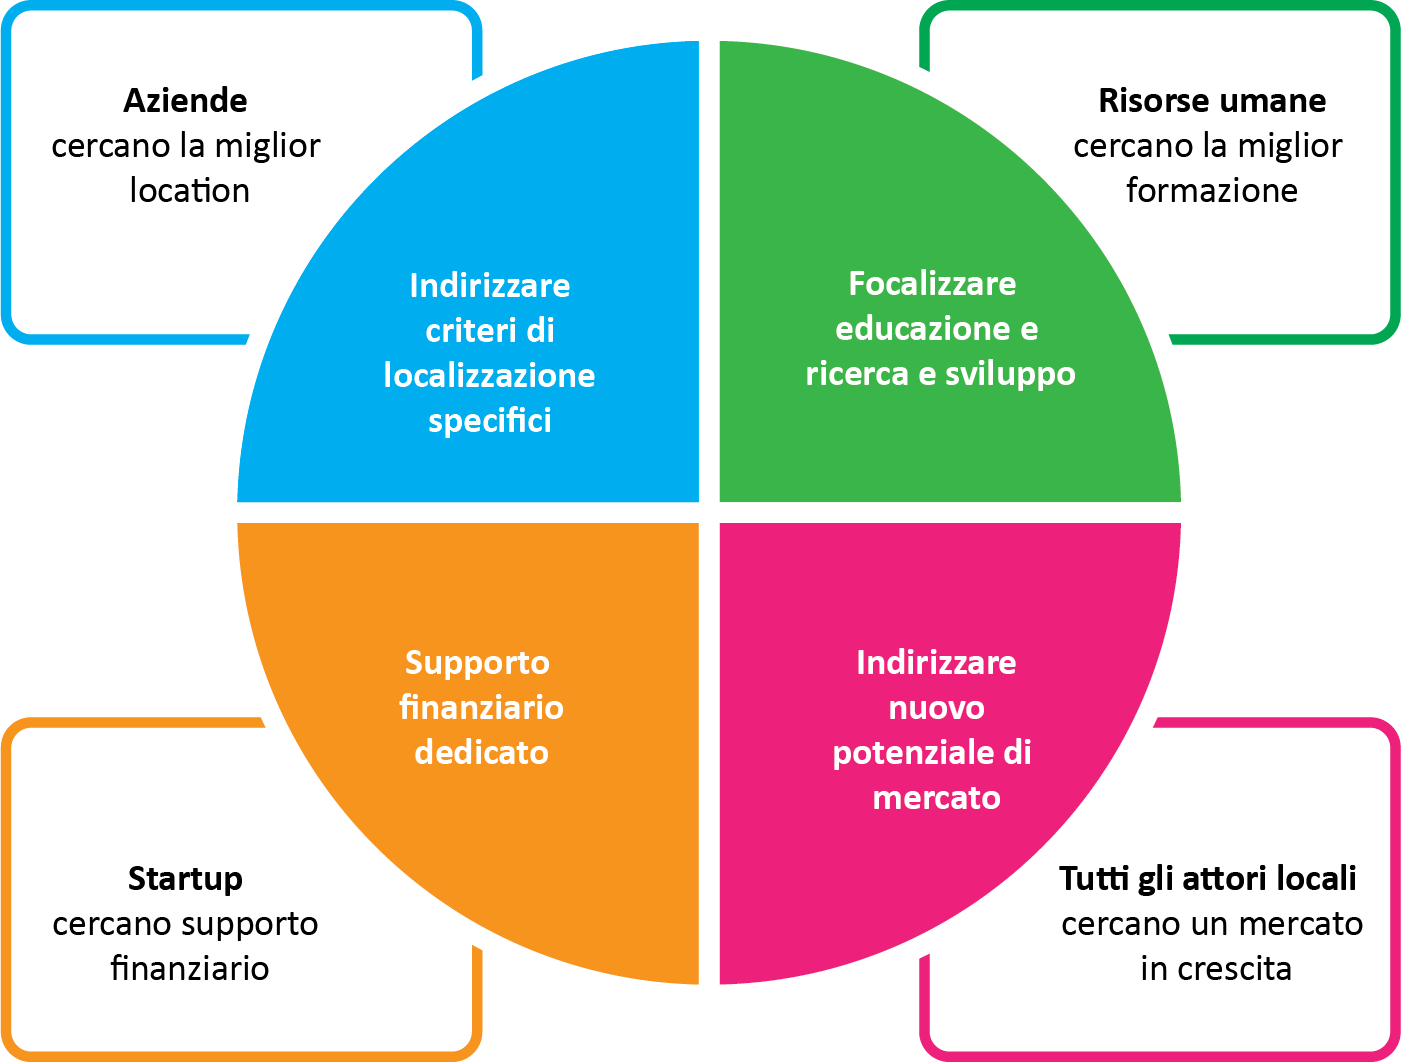
\includegraphics[scale=0.37]{immagini/sss_graph.png}
	\caption{Parti coinvolte e ruoli nella Smart Specialisation Strategy.}
	\small{\textbf{Fonte:} \url{https://www.slideshare.net/TCINetwork/8-clac-18-junefrederic-miribel}}	
	\end{center}
\end{figure}
\subsubsection{L'approccio di Lab Network alla S.S.S.}
\lab{} mette a disposizione un portale dedicato dove aziende e fabbricanti possono comunicare scambiando sapere tecnologico e progetti nell'ottica innovativa dell'economia condivisa.
\\
L'\gls{SWOT} (Strengths, Weakness, Opportunities, Threats) condotta da \lab{} sulla realtà delle PMI venete, evidenzia come ci sia uno scarso utilizzo di tecnologie dell'informazione e della comunicazione (ICT), scarsa disponibilità di laboratori di proprietà, bassi investimenti in ricerca, difficoltà a sviluppare progetti innovativi e ridotta capacità di reperire risorse e professionalità necessarie. 
L'obiettivo di \lab{} è quello di colmare queste lacune mettendo a disposizione alle aziende un'area di lavoro a costi contenuti dove poter utilizzare i principali strumenti di innovazione digitale come: stampanti 3D, kit elettronici, macchine a controllo numerico, frese digitali e taglio laser. Tutto questo può essere definito come un laboratorio per studiare la fase prototipale.
\\
In pratica \lab{} vuole contribuire a portare l'innovazione e la tecnologia all'interno delle PMI che ancora non si sono interfacciate a questo ``nuovo mondo''.